\documentclass[11pt]{article}
\usepackage{authblk}
\usepackage{arydshln}
\usepackage[margin=2cm]{geometry}
\usepackage{adjustbox}
\usepackage{multirow}
\usepackage{arydshln}

\newcommand{\beginsupplement}{%
        \setcounter{table}{0}
        \renewcommand{\thetable}{S\arabic{table}}%
        \setcounter{figure}{0}
        \renewcommand{\thefigure}{S\arabic{figure}}%
     }
%\geometry{a4paper, portrait, margin=1.2in}

\setlength{\parskip}{\baselineskip}%
\setlength{\parindent}{30pt}%
\linespread{2}

\title{\textbf{Estimating the parameters of selective sweeps from patterns of genetic diversity in the house mouse genome}}
\author[1,*]{Tom R. Booker}
\author[1]{Brian Charlesworth}
\author[1]{Peter D. Keightley}
\affil[1]{Institute of Evolutionary Biology, University of Edinburgh, Edinburgh}
\affil[*]{\emph{t.r.booker@sms.ed.ac.uk}}






\begin{document}
\maketitle
\begin{abstract}


\end{abstract}

%%%%%%%%%%%%%%%%%%%%%%%%%%%%%%%%%%%%%%%%%%%%%%%%%%%%
%
%  #   #    #  #####  #####  ######
%  #   ##   #    #    #   #  #    #     
%  #   # #  #    #    #####  #    #
%  #   #  # #    #    #  #   #    #           
%  #   #   ##    #    #   #  #    #  
%  #   #    #    #    #   #  ######    
%
%%%%%%%%%%%%%%%%%%%%%%%%%%%%%%%%%%%%%%%%%%%%%%%%%%%%

\section*{Introduction}

In the past 30 years of population genetic research it has become clear that natural selection shapes patterns of nucleotide diversity across the genomes of many species \citep{RN154, RN117}. Because genetically linked sites do not evolve independently, selection acting at one site may have consequences for another. The consequences of selection at linked sites are intrinsically linked to the frequency and strength of selected mutations as well as, crucially, the rate of recombination (REF DUMP). Two main modes of selection at linked sites have been identified; selective sweeps caused by the spread of advantageous mutations and background selection caused by the removal of deleterious variants. The two processes are related and can both potentially explain the positive correlations between nucleotide diversity and recombination rate reported in many species \citep{RN117}. However, the proportion of nonsynyonomous substitutions attributable to adaptive evolution ($\alpha$) is typically high (50\%) (\citealt{RN215}; but see \citealt{RN352} for caveats), suggesting that selective sweeps may play a substantial role in shaping nucleotide diversity across the genomes of many species.

Selective sweeps have been subject to rigorous population genetic research \citep{RN124, RN226, RN278, RN235}. The classic footprint of a selective sweep is a trough in nucleotide diversity at neutral sites surrounding substitutions. Reductions in nucleotide diversity caused by selective sweeps are related to the strength of selection acting on advantageous mutations as well as the frequency with which they arise. Taking advantage of this, \cite{RN277} used a model of selective sweeps to estimate the frequency and strength of advantageous mutations in \textit{Drosophila melanogaster} by fitting the positive correlation between recombination rate and nucleotide diversity. At the time of their analysis, the theory of background selection was in its infancy and models combining the effects of background selection and sweeps had not been developed. However, the effects of background selection are expected to be ubiquitous across the genome \citep{RN116, RN274, RN120}, and studies, conceptually similar to Wiehe and Stephan's (1993), have shown that controlling for background selection is highly important when parametrizing sweep models from patterns of nucleotide diversity \citep{RN323, RN274}.

Because both selective sweeps and background selection act to reduce nucleotide diversity, it has proven difficult to distinguish their effects using population genetic data \citep{RN339}. A number of different approaches have been taken to tease apart the effects of the two processes. For instance, \cite{RN167} showed that, on average, there is a trough in diversity around recent nonsynonymous protein-coding substitutions in \textit{Drosophila melanogaster} but not around synonymous ones. This pattern is strongly suggestive of selective sweeps, so they \citep{RN167} fitted a sweep model to the trough they observed and estimated that strongly advantageous mutations ($2N_es$ $\approx$ 5,000) occur in the fruitfly's genome.  In the house mouse, there is also a trough in diversity around recent nonsynonymous substitutions, but an almost identical trough is observed around synonymous substitutions, furthermore a similar trough is observed around even randomly selected synonymous and nonsynonymous sites in the genome \citep{RN122}. This all, perhaps, suggests that the reductions in diversity caused by selection at linked sites extend beyond the average distance separating nonsynonymous substitutions, so that the methods employed by \cite{RN167} are not effective in mice \citep{RN122}. For both classes of elements, however, values of $\alpha \geq 0.19$ have been reported for both classes of elements \citep{RN122} and background selection alone cannot fully explain the troughs in diversity (\citealt{RN122}, Booker and Keightley \textit{Unpublished}), suggesting that selective sweeps do contribute to the observed patterns.

In Chapter 3, we sought to tease apart the contribution of BGS and SSWs to patterns of diversity in mice. We estimated distributions of fitness effects (DFEs) for both harmful and advantageous mutations occurring in multiple classes analysing the distribution of derived allele frequencies (referred to as the unfolded site frequency spectrum, hereafter uSFS). The methods that we used, and related approaches, rely on the assumption that selected mutations segregate in populations of interest, such that they affect the shape of the uSFS. Using simulations, we found that neither BGS nor SSWs given the parameters we estiamtes could explain troughs in diversity observed around protein-coding exons or conserved non-coding elements (CNEs)
Using simulations, we showed that the parameters of the DFE we obtained were unable to explain the troughs in diversity around protein-coding exons, but were able to explain the troughs around conserved non-coding elements. A possible explanation for our inability to explain the observed patterns is that advantageous mutations have large effects effects on fitness and may not be detectable by analysis of the uSFS. occur in protein-coding regions have, on average, larger effects on fitness that those occurring in regulatory regions which may affect the power to 

In this study, we use a model of selective sweeps to estimate the strength and frequency of advantageous mutations that occur within protein-coding exons and regulatory elements. Using simulations, we show that the selection parameters that explain the troughs in diversity are out of the range detectable by analysis of the uSFS.  We find that, as expected \textit{a priori}, the strength of selection acting on protein-coding exons is far greater than that acting in regulatory elements. Finally, using a simple model of the fitness change brought about by adaptive evolution, we show that, despite adaptation occurring more frequently in regulatory regions, adaptation in protein-coding regions may contribute more to phenotypic evolution in mice.

%%%%%%%%%%%%%%%%%%%%%%%%%%%%%%%%%%%%%%%%%%%%%%%%%%%%
%
% #   #  ####  #####  #   #  ####    ####
% ## ##  #       #    #   #  #   #   #  
% # # #  ###     #    #####  #   #   ####
% #   #  #       #    #   #  #   #      #        
% #   #  #       #    #   #  #   #      #
% #   #  ####    #    #   #  ####    ####
%
%%%%%%%%%%%%%%%%%%%%%%%%%%%%%%%%%%%%%%%%%%%%%%%%%%%%
\section*{Materials and Methods}


	\subsection*{Simulations}
	
	We generated simulated datasets using the forward-time simulation package SLiM (v1.8; \citealt{RN148}). We simulated the evolution of 1Mbp chromosomes containing 20 evenly spaced out `genes`. Each `gene` consisted of 10 100bp exons, separated by 1Kbp of neutrally evolving intronic sequence. Nonsynonymous mutations were modelled as 75\% of mutations occurring in exons, the remaining 25\% were strictly neutral (i.e. synonymous sites). We varied the $\gamma_a$ and $p_a$ parameters across simulations, but kept the product $\gamma_a p_a$ equal to 0.1. We based this value of $\gamma_a p_a \approx 0.1$ on a recent study in \textit{Drosophila melanogaster} \citep{RN321}. All simulations incorporated the same gamma dDFE ($\beta$ = 0.2 and $\hat{\gamma_d}$ = -1,000). The advantageous mutation parameters we simulated are listed in Table \ref{polyDFE}. 	The population-scaled mutation and recombination rates (i.e. $\theta$ = \emph{$4N_{e}\mu$} and $\rho$ = \emph{$4N_{e}r$}, respectively) were set to 0.01. Populations of $N$ = 1,000 diploid individuals were simulated for an initial burn-in of 10$N$ generations to establish equilibrium conditions. After the burn-in, 20 haploid chromosomes were sampled every 2$N$ generations for a further 100$N$ generations. We performed 10 simulation replicates for each set of selection parameters (Table \ref{polyDFE}). Across simulation replicates, time-points and loci we extracted the simulated nonsynonymous and synonymous sites, giving uSFS data for 10,000 `genes'. We sampled the set of 10,000 `genes' with replacement 100 times, collating the nonsynonymous and synonymous site uSFSs for each replicate.


	\subsection*{Analysis of the uSFS}

	
	We estimated the DFEs in our simuations by analysing the uSFS using the methods of \cite{RN354} as implemented in the polyDFE (v1.1) package. PolyDFE fits an expression for the uSFS expected in the presence of both advantageous and deleterious mutations to data from putatively neutral and selected classes of sites, by maximum likelihood. The neutral class uSFS is used to determine distortions to the uSFS caused by processes such as selection at linked sites and a history of population size change. In addition, polyDFE corrects for polymorphism misattributed to divergence, mutation rate variability and error in assigning sites as ancestral/derived. \cite{RN354} performed extensive simulations and showed that accurate estimates of the parameters for both deleterious and advantageous mutations can be obtained using their methods. However, there are a range of parameters that they did not test which may be biologically relevant, specifically when advantageous mutations are strongly selected, but infrequent.

	 We analysed our simulated uSFSs using polyDFE choosing Model C (a gamma dDFE and a discrete class of advantageous mutations) and either including or not  between-species divergence. We analysed the uSFS for simulated nonsynonymous using simulated synonymous sites as the neutral reference class. For each DFE tested we analysed 100 bootstrap samples of the simulation data.
 
 	
	\subsection*{Model of Recurrent Sweeps with Background Selection}
%Background selection (BGS) is often modelled as the reduction in diversity experienced by a focal neutral site caused by deleterious mutations occurring at linked selected sites. An approximation for the reduction in diversity caused by background selection:
%\begin{equation}
%B = \frac{N_{e}}{N_{0}} \approx exp\Bigg[- \sum \limits_{x} \int \limits_{0}^1 \frac{u_{x}f_x(t)\mathop{dt}}{t \Big( 1 + \frac{(1-t)r_{i,j}}{t} \Big)^2} \Bigg]
%\end{equation}
%Where the sum is over all linked selected sites, the integral is over the distribution of fitness effects for deleterious mutations, \emph{$u_{x}$} is the deleterious mutation rate, \emph{t} is the reduction in fitness for heterozygotes (assumed to be \(\frac{s}{2}\) ), $r_{x,y}$  is the recombination distance between the focal neutral site and the selected site and $f_x(t)$ is the proportion of sites in the DFE with selection coefficient $t$.

%	Background selection (BGS) and selective sweeps (SSWs) are processes that induce coalescence at linked neutral sites. Provided that the effects of both processes are relatively weak as compared to drift, the effects of the two can simply be summed (Kim and Stephan 2001). Furthermore, if it is assumed that harmful mutations and is far more frequent than SSWs, BGS may reduce the population scaled mutation rate, and thus the rate of selective sweeps. Under the above assumptions, the combined effect of the two processes have on levels of genetic diversity can be modelled as the following:
	
	\cite{RN323} gave expressions for the expected neutral diversity given the combined effects of background selection (BGS) and selective sweeps (SSWs). They assumed that the effects of BGS and SSWs act independently so that their effects can simply be summed. However, background selection causes a reduction to the effective population size ($N_e$) at a neutral locus, $j$ by some fraction $B_j$. The rate and fixation probability of new advantageous mutations is dependant upon $N_e$, so we scale the rate of sweeps by $B_j$ in a modified version of the model used by \cite{RN323},
	
\begin{equation}
\label{jointApprox}
\frac{\pi_{j}}{\pi_{0}} \approx  \frac{1}{B_{j}^{-1}  + B_{j}2N_eP_{sc,j}}.
\end{equation}
	Where $\pi_j$ is neutral genetic diversity observed at neutral site \textit{j} and $\pi_0$ is diversity expected in the absence of selection at linked sites. The $P_{sc,j}$ term is the reduction in coalescence times at site \textit{j} caused by the effects of SSWs,

\begin{equation}
\label{singleClass}
P_{sc,j} \approx V_a \tau\gamma_a^{\frac{-4r_{i,j}}{s}} 
\end{equation}
The term $V_{a} = 2 \mu p_{a} \gamma_{a}$ is the rate of sweeps per generation, where $\mu$ is the per-base pair per generation mutation rate, $p_a$ is the fraction of new mutations occurring within a focal element that are advantageous and $\gamma_a$ is the scaled selection coefficient of a new mutation ($2N_es_a$) (Kimura and Ohta?). $\tau$ is the number of selected sites in a functional element. The recombination fraction between a functional element ($i$) and the focal neutral site is $r_{i,j}$. When assuming that recombination proceeds solely by crossing over $r_{i,j}$ is simply the product of the physical distance ($d_{i,j}$) and the local crossing-over rate ($r_c$). When incorporating gene conversion, we use Equation 1 from  \cite{RN361}:
 		\begin{equation}
		\label{geneConversion}
		r_{i,j} = d_{i,j} r_c + g_c d_g \Bigg( 1 - e ^{-\frac{d_{i,j}}{d_g}} \Bigg)
		\end{equation} where $g_c$ is the rate of gene conversion and $d_g$ is the mean gene conversion tract length, assuming that the distribution of tract lengths is exponential. When applying Equation \ref{geneConversion} we use $g_c = \kappa r_c$ where $\kappa$ is the ratio of the crossing over rate to the gene conversion rate.
	
	There is evidence that the distribution of fitness effects for advantageous mutations is beneficial from both theoretical \cite{RN362} Griffiths REFS) and empirical studies (DATA Papers?). IT is straightforward to incorporate an exponential distribution of advantageous mutation effects to Equation 3
		\begin{equation}
		\label{exponential}
P_{sc,j} \approx \int \limits_{0}^{\infty} f_x(\gamma) V_a \tau\gamma_a^{\frac{-4r_{i,j}}{s}} \mathop{d\gamma}
		\end{equation}

	
	We estimated $\gamma_a$ and $p_a$ by fitting Equation \ref{jointApprox} to the relationship between nucleotide diversity and distance to functional elements using non-linear least squares with the \emph{lmfit} (0.9.7) package for Python 2.7. When analysing the mouse data, see below, we compared the fit of Equation \ref{jointApprox} incorporating either one or two discrete classes of beneficial mutations (Equation \ref{singleClass}) or the exponential distribution (Equation \ref{exponential}) using Aikieke's Information Criterion (AIC).
	
	
%	When fitting Equation \ref{jointApprox} an estimate of $\pi_0$ is required. However, $\pi_0$ is ot easily estimated because a large proportion of the genome is likely influenced by selection at linked sites. The troughs in diversity around exons an CNEs plateau at value that are reduced below the neutral expectation (Booker and Keightley Unpublished). This is because selection at multiple linked elements acts to reduce putatively neutral diversity. Our estimates of \textit{B} from the simulation data plateau at \approx 0.95. A point estimate of $pi_0$ could 

	\subsection*{Analysis of Mouse Data}

	We analysed patterns of genetic diversity in 10 wild-caught \textit{M. m. castaneus} individuals, first reported by \cite{RN122}. Breifly, \cite{RN122} sequenced individual genomes to high coverage ($\approx$ 30x) using Illumina paired-end reads, which were mapped to the mm9 mouse reference genome using BWA. Variants were called using a Samtools pipeline. Note that we only analyse SNP data in this study, insertion/deletion variants are not included. For further details of the sequencing and variant calling methods see \cite{RN122}. Protein-coding exons present in the version 67 of the Ensembl annotation database and the locations of conserved non-coding elements identified by \cite{RN122} using an alignment of placental mammals were used in this study.

	From the edges of exons (CNEs), polymorphism data and divergence to the rn4 rat reference genome were extracted for non-CpG sites in windows of 1Kbp (100bp) extending to distances of 100Kbp (5Kbp). Analysis windows were then binned based on genetic distance to the focal element using either the LD-based recombination map for \textit{M. m. castaneus} constructed by \cite{RN340} or the pedigree-based genetic map constructed using common lab strains of \textit{M. musculus} by \cite{RN232}. Because LD-based and pedigree based recombination maps have different benefits and drawbacks (discussed below), we perform all analyses in parallel, assuming both of these recombination maps.

	Recombination proceeds via crossing-over or gene conversion, but the above formulae (Equations \ref{singleClass} and \ref{exponential}) assume that genetic distance is solely a product of the local crossing-over rate and the physical distance. We incorporated gene conversion into genetic distance by calculating $r_{i,j}$ in Equations \ref{singleClass} and \ref{exponential} using Equation 1 from \cite{RN361}
		\begin{equation}
		\label{geneConversion}
		r_{i,j} = d_{i,j} r_c + g_c d_g \Bigg( 1 - e ^{-\frac{d_{i,j}}{d_g}} \Bigg)
		\end{equation}
	where $d_{i,j}$ is the physical distance between a focal neutral site and a selected site, $r_c$ is the rate of recombination by crossing-over, $g_c$ is the rate of non-crossing over gene conversion and $d_g$ is the mean length of a gene conversion tract. This assumes that the distribution of gene conversion tract lengths is exponential. We assumed a mean tract length of 144bp and that the gene conversion rate was 10.5\% of the local crossing-over rate (Paigen \textit{et al.} 2008).

	We assume the point mutation rate to be $5.4 \times 10^{-9}$ \citep{RN228}.
 	The mean length of a protein-coding exon is 151bp.
 	The mean length of a conserved non-coding exon is 51bp.
	
	
	\subsection*{Estimates of \textit{B}} 
 
 	Background selection contributes to the troughs in diversity around both protein-coding exons and CNEs (Halligan et al 2013; Booker and Keightley Unpublished). Because of this, we required estimates of the effect of background selection on neutral diversity, \textit{B}, to fit as a covariate when fitting Equation \ref{jointApprox} to the diversity troughs. There are formulae for calculating \textit{B} given the DFE as well as mutation and recombination rates \citep{RN157, RN206}, but these over-predict the effects of BGS when purifying selection is weak ($\gamma_d < 1$) (Good and Desai; Gordo et al). Since weakly selected mutations comprise a large portion of the DFEs we obtained previously, we opted to obtain estimates of \textit{B} from simulations. In Chapter 3, we used simulations to estimate the contribution of background selection to patterns of nucleotide diversity around both protein-coding exons and CNEs. These simulations incorporated recombination rate variation, the actual distribution of functional elements in the genome and dDFEs specific to each of the functional elements analysed. By extracting diversity as a function of genetic distance to both protein-coding exons and CNEs from these simulations, we obtained estimates of \textit{B} that can be used when fitting Equation \ref{jointApprox}.
 	
 	The simulations we used to estimate $B$ were the same as those we used in Chapter 3, except that we increased the number of simulation replicates from 2,000 to 6,000. To obtain smoothed $B$ values we fit Loess curves to the simulation data using R (v3.4.2). We fit Loess curves using a span of 0.2 and used the number of sites contributing to each analysis bin as weights.

%%%%%%%%%%%%%%%%%%%%%%%%%%%%%%%%%%%%%%%%%%%%%%%%%%%%
%
% ####   ####  #####  #   #  #     #######  #####
% #   #  #     #      #   #  #        #     #
% ## #   ###   #####  #   #  #        #     #####
% # #    #         #  #   #  #        #         #
% #  #   #         #  #   #  #        #         #
% #   #  ####  #####  #####  #####    #     #####
%
%%%%%%%%%%%%%%%%%%%%%%%%%%%%%%%%%%%%%%%%%%%%%%%%%%%%

\section*{Results}

\begin{sidewaystable}
\caption{Positive selection parameter estimates obtained by analysis of the uSFS for simulated poplations. }
\begin{tabular}{ccccccc}

\toprule
 \multirow{2}{*}{Divergence \footnote{+/- indicates whether or not divergence was included when analysing the uSFS} } & \multicolumn{2}{c}{$\gamma_a$} & \multicolumn{2}{c}{$p_a$}  & \multirow{2}{*}{$\gamma_a p_a$} & Prop.\\
 	&    \textit{Simulated} & \textit{Estimated} & \textit{Simulated} & \textit{Estimated} &  &  Significant \footnote{The proportion of bootstrap replicates where a full DFE gave a significantly better fit than a model containing just deleterious mutations}\\
\midrule
         + &    \multirow{2}{*}{10} & 11.2 [5.60 - 20.0] &  \multirow{2}{*}{0.010000} & 0.00856 [0.00440 - 0.0199] &  0.0954 [0.0838 - 0.115] &  1.00 \\
         - &     & 3.97 [1.13 - 27.2] &   &         0.0201 [0.00472 - 0.0706] &  0.0828 [0.0616 - 0.155] &               1.00 \\
         + &   \multirow{2}{*}{20} &           16.6 [9.20 - 37.4] &  \multirow{2}{*}{0.005000} &  0.00568 [0.00241 - 0.0107] &  0.0949 [0.0822 - 0.108] & 1.00 \\
         - &    &        19.9 [2.90 - 37.4] &   & 0.00532 [0.00289 - 0.0207] &  0.106 [0.0454 - 0.193] &  0.97 \\
         + &   \multirow{2}{*}{50} &   37.4 [21.6 - 41.8] &  \multirow{2}{*}{0.002000} & 0.00257 [0.00202 - 0.00467] &  0.0951 [0.0809 - 0.106] & 1.00 \\
         - &    &   37.3[1.87 - 65.5] &  & 0.00266 [0.00125 - 0.0146] &  0.0717 [0.0112 - 0.145] &  0.86 \\
         + &   \multirow{2}{*}{100} &   37.43 [37.4 - 1530] &  \multirow{2}{*}{0.001000} &        0.00249 [0.0000738 - 0.00283] &   0.0938 [0.0795 - 0.107] &  1.00 \\
         - &    &  0.323 [0.0371 - 1.25] &   &  0.00259 [0.000525 - 0.0941] &  0.00102 [0.0000620 - 0.0137] & 0.00 \\
         + &  \multirow{2}{*}{200} &  37.4 [37.4 - 1,700] &  \multirow{2}{*}{0.000500} & 0.00251 [0.000220 - 0.00283] &     0.0947 [0.0738 - 0.106] & 1.00 \\
         - &   &            0.272 [0.00546 - 1.911] &   &                     0.0122 [0.000690 - 0.138] &  0.00310 [0.000104 - 0.0294] & 0.07 \\
         + &  \multirow{2}{*}{400} & 37.4 [32.7 - 37.4] &  \multirow{2}{*}{0.000250} & 0.00245 [0.00199 - 0.00283] &  0.0919 [0.0776 - 0.102] & 1.00 \\
         - &   & 12.3 [0.287 - 66.6] &   &  0.00212 [0.000783 - 0.0104] &  0.0338 [0.000250 - 0.0984] & 0.22 \\
         + &  \multirow{2}{*}{800} & 37.4 [32.9 - 37.4] &  \multirow{2}{*}{0.000125} & 0.00222 [0.00186 - 0.00264] &       0.0831 [0.0701 - 0.0936] & 1.00 \\
         - &   & 1.75 [0.111 - 43.0] &   &  0.00240 [0.000343 - 0.0293] &  0.0134 [0.0000515 - 0.0649] & 0.12 \\
\bottomrule
\end{tabular}
  \label{tab:advMuts}

\end{sidewaystable}

\subsection*{Estimating selection parameters from the uSFS of simulated data}

	Parameters of the DFE can be estimated directly from unfolded site frequency spectra (uSFS) if selected mutations are segregating in populations of interest (REFS). It has been repeatedly demonstrated that parameters of the DFE for deleterious mutations (dDFE) can be accurately estimated from population genetic data. It has also been shown that the parameters of advantageous mutations can also be estimated from the uSFS \citep{RN210, RN354}, but it has been argued that strongly selected advantageous mutations, which may contribute little to standing variation, will be undetectable by such methods \citep{RN323}. In this study, we confirm this verbal argument using simulations, showing that accurate estimation of positive selection parameters does indeed depend on the strength and relative frequencies of advantageous mutations.
	
	We used forward-in-time simulations that incorporated linkage, because selection at linked sites can distort the uSFS in ways that likely affect real data and thus cannot be ignored. For each set of advantageous mutation parameters, we simulated 10Mbp of gene-like sequences giving a total of 7.5Mbp of nonsynonymous sites and 2.5Mbp of synonymous sites which we used to construct the uSFS for 20 haploid individuals. This sample size and quantity of data is fairly typical of population genomic studies (REFS). Using these data we estimated the parameters of selection using polyDFE, an implementation of the methods of Tataru \textit{et al} (2017). These methods allow the simultaneous estimation of the dDFE and positive selection parameters, taking into account distortions in the uSFS caused by, for example, the effects of demography and selection at linked sites. 

	Consistent with \cite{RN354}  we found that polyDFE gave estimates of the dDFE were very accurate. In particular, the shape parameter of the gamma dDFE was estimated with precision. Overall, the estimation performed most poorly when divergence was included, but only a dDFE was inferred. These results replicate the findings of \cite{RN354} and further emphasize the importance of specifying a full DFE model when making inferences of selection from the uSFS. 
	
	 We analysed the uSFS from our simulated populations and found that when advantageous mutations are relatively frequent ($p_a$ $>$ 0.0005), but weakly selected ($\gamma_a$ $<$ 100), both $\gamma_a$ and $p_a$ parameters can be estimated with precision (Table REF). However, we found that when advantageous mutations were infrequent but strongly selected ($\gamma_a$ $\geq$ 100 and $p_a$ $\leq$ 0.0005) the parameters were very poorly estimated. Across all simulated datasets, when we included divergence in the analysis, the product $\gamma_a p_a$ was accurately estimated (Table REF) and likelihood ratio tests never failed to detect the presence of advantageous mutations in the uSFS. When we excluded divergence from the analysis, however, the product  $\gamma_a p_a$  was poorly estimated when $\gamma_a \geq 100$ and likelihood ratio tests typically failed to detect positive selection (Table REF).
	
	Across different sets of simulations, the strength of selection differed (ranging between $\gamma_a$ = 10 and $\gamma_a$ = 800), but the product $\gamma_a p_a$, which is expected to be directly proportional to the rate of sweeps, was always equal to 0.1. All simulations were subject to the same dDFE, so the extent of background selection should be fairly similar. We found that selection at linked sites reduced synonymous site diversity below the expectation value of 0.01 in all simulations (Table \ref{tab:summaryStats}),  but as the strength of selection acting on advantageous mutations increased, diversity at linked sites decreased (reflected in in the decreasing values $\pi/\pi_0$ shown in Table \ref{tab:summaryStats}). As expected, the relative fixation rate of nonsynonymous mutations (meausured using  $dN/dS$ ) did not vary systematically across simulations (Table \ref{tab:summaryStats}).
	
	The number of fixed, advantageous mutations carries information on the compound parameter $\gamma_a p_a \mu$ (Kimura and Ohta 1971), which will be embedded within between species divergence at selected sites. Without further information from polymorphism data, this compound parameter cannot be disentangled by analysis of the uSFS. Across our simulations, the rate of sweeps did not vary, but nucleotide diversity at neutral, synonymous sites did; as the scaled strength of selection increased, synonymous site diversity decreased (Table \ref{tab:summaryStats}). This all suggests that when advantageous mutations are strongly selected, but rare, patterns of nucleotide diversity carry information that is not present in the unfolded site frequency spectrum.

\subsection*{Patterns of genetic diversity around protein-coding exons and conserved non-coding elements}

\begin{figure}[h]
   \centering      
   \noindent\makebox[\textwidth]{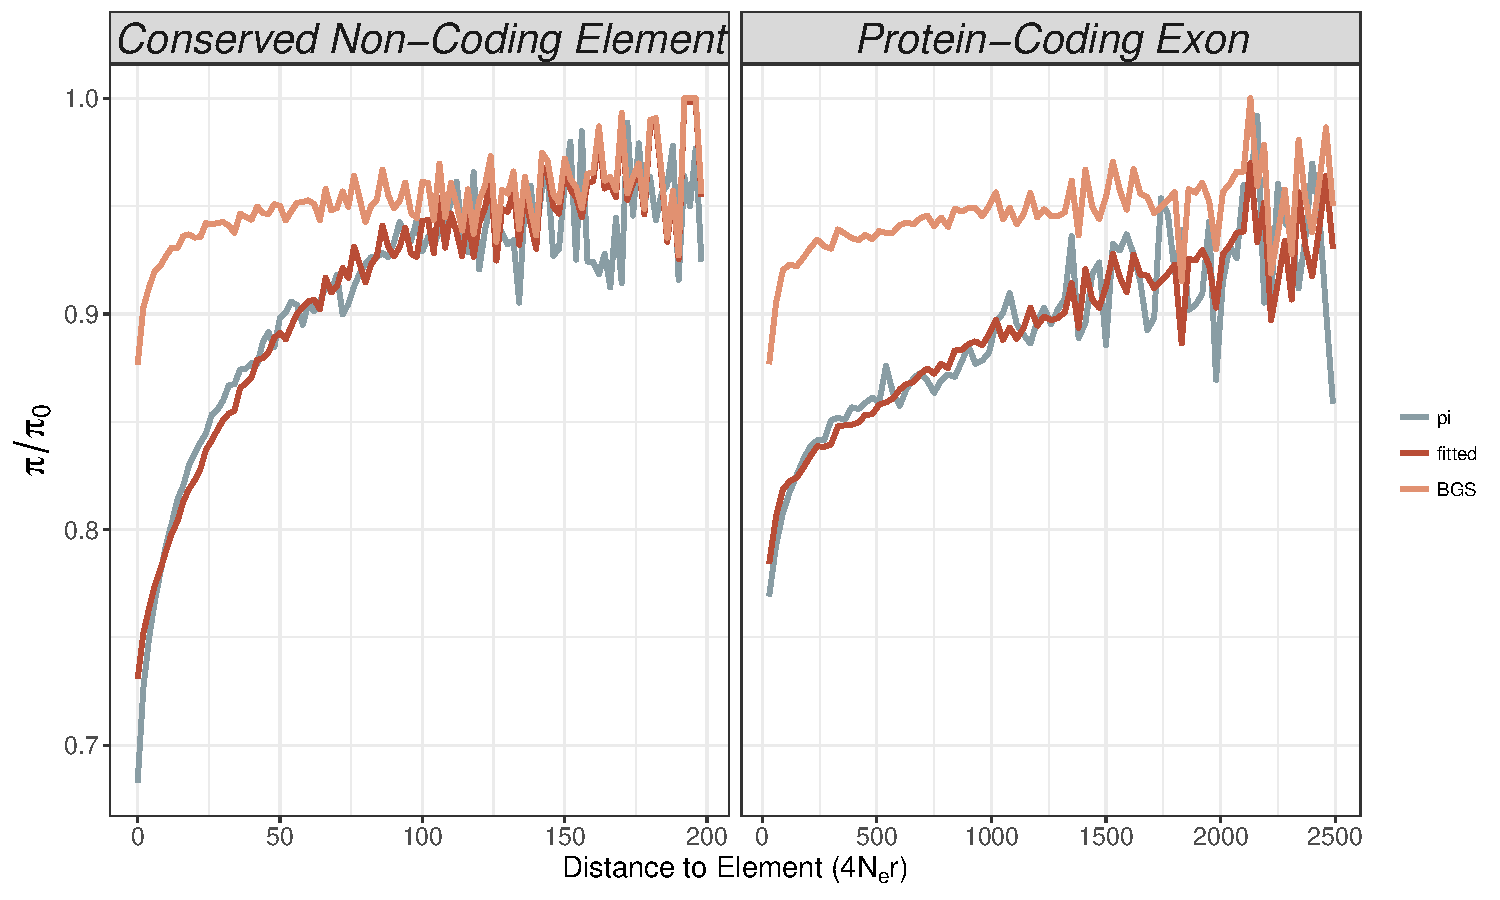
\includegraphics[width=\textwidth]{/Users/s0784966/PhD/Coding/Estimate_selection_from_troughs/Presentation/data_analysis_singleClass.pdf}}
 \caption[The ]
 
 \label{fig:1}
\end{figure}

	Recombination rates can be estimated in various ways, which have different pros and cons. For instance, the population-scaled recombination rate ($\rho$) can be inferred from a relatively small sample of unrelated individuals at very fine-scales using patterns of linkage disequilibrium (LD) (REVIEW?). However, selection at linked sites influences local LD and may therefore affect recombination rate estimates obtained in this way (REF?). Alternatively, direct estimates of the recombination rate ($r$) can be obtained from crossing experiments, but to achieve sufficient power to generate recombination maps a very large number of individuals need to be genotyped, which has typically precluded the use of whole-genome re-sequencing, limiting resolution. In summary, high resolution recombination maps can be generated using patterns of LD, but these may be biased by selection at linked sites, while unbiased recombination maps may be generated using crosses, though these typically have low resolution. When analysing patterns of genetic diversity using a model of selection at linked sites, the way in which recombination rate estimates were obtained may, therefore, affect parameter estimates.

	In this study, we analysed patterns of genetic diversity in \textit{M. m. castaneus} and calculated genetic distances assuming either the high resolution recombination map constructed from LD by \cite{RN340}(the \textit{castaneus} map) or the pedigree-based map of \cite{RN232} (the Cox map). The choice of recombination map had a substantial effect on patterns of nucleotide diversity. We found that, in the immediate flanks of both exons and CNEs, diversity was lower when assuming the LD-based \textit{castaneus} map than when assuming the pedigree-based Cox map (Figure X). This difference is consistent with the idea that regions of the genome close to functional elements, where the effects of BGS and/or SSWs are strongest, and which exhibit reduced diversity, may yield downwardly biased estimates of the recombination rate. An alternative explanation is that the Cox map, which lacks resolution, does not fully capture regions of low recombination rate, so analysis windows that are tightly linked to functional elements may appear less tightly linked. An additional caveat is that in order to scale  recombination rate estimates in the Cox map to $\rho$ values, we assumed a single $N_e$ for the entire genome, though $N_e$ may very well vary across the genome. However, genetic diversity  plateaus at a higher level when assuming the \textit{castaneus} map, suggesting that the Cox map may not capture some of the highly recombining portions of the genome. The choice of recombination rate estimates will, therefore, have an impact on the parameters of selection inferred from the patterns of diversity. Throughout the rest of the paper, we present, in parallel, the results of analyses based on the \textit{castaneus} map with those based on the Cox map.

	\subsection*{Diversity expected in the absence of selection, $\pi_0$}

	A key parameter in Equation \ref{jointApprox} is $\pi_0$, the nucleotide diversity expected in the absence of the effects of selection at linked sites. This parameter is very difficult to estimate and may even prove unobservable in real data given the ubiquity of the effects of selection at linked sites \citep{RN357}. However, an estimate of $\pi_0$ is required to fit the troughs in diversity. When fitting the data, the value of this parameter we assumed depended on which recombination map we assumed and which functional element was being analysed. The distribution of functional elements surrounding protein-coding exons and CNEs differs, which will affect the level at which nucleotide diversity plateaus surrounding those elements, as the effects of selection at linked sites will differ between the two. This may explain why the level at which diversity plateaus around the two classes of elements, as can be seen in Figure \ref{fig:1}.
	The reductions in diversity caused by selective sweeps occuring at linked elements will differ around CNEs and protein-coding exons as the distribution of function
	unobservable in the patterns of nucleotide diversity around both classes of elements analysed in this study, as even where neutral diversity plateaus, it is reduced below its expected 

\subsection*{Parameters of selective sweep obtained from patterns of nucleotide diversity}

	By fitting Equation \ref{jointApprox} to the troughs in diversity surrounding protein-coding exons and CNEs, we were able to estimate that very strongly selected mutations may occur in both elements. Regardless of which recombination map we assume, selection coefficients for mutations occurring in exons were order of magnitude greater than CNEs. Comparing selection parameters obtained assuming the Cox ans \textit{castaneus} maps highlight a 

	What was the effect of including background selection or not?
	
	If we assume a long-term effective population size of 420,000 for \textit{M. m. castaneus}, we estiamte that selection coefficients in natural popuations of $\approx 0.01$


	We compared the fit of different models for the DFE for advantageous mutations, but found that a single class of effects gave the best fit. Using AIC, we compared the fit of one or two classes of discrete effects as well as the exponential distribution. In the case of protein-coding exons a single class of effects or an exponential distribution gave similar fits to the data, as judged by differences in AIC, regardless of whether we used the \textit{castaneus} or Cox maps to estimate genetic distances. In the case of CNEs, on the other hand, a single class of advantageous mutations was supported in when analysing using the Cox distances, but two class of effects were strongly supported when using the \textit{castaneus} map. 

	We estimated the parameters of a model of recurrent selective sweeps acting in two different classes of functional elements in \textit{M. m. castaneus}. We compared parameters obtained when incorporating gene conversion and background selection.
	
	Using  Equation \ref{geneConversion} we incorporated gene conversion into the analysis. However, given estimates of gene conversion parameters in mice, that it did not substnatially influence the analysis. We assumed gene conversion parameters estimated by \cite{RN263}, but incorporating these did not influence the selection parameters. In that study, the ratio of non-crossover gene conversion to crossing-over (NC/CR) was estimated to be 0.105, while gene conversion tracts measuring 9-279bp were detected. When assuming the center of this range (144bp) as the mean tract length and a NC/CR ratio of 0.105, gene conversion did not affect the selection parameter estimates. However, the gene conversion parameters estiamted by \cite{RN263} were based on a small number of observations and the true parameters may be quite different. I
	This is not particularly surprising since the physical distances analysed are far greater than the mean tract length assumed.  

Estimates of selection obtained for protein-coding regions were an order of magnitude higher than those obtained for conserved non-coding elements. 






\begin{table}[h]
\caption{Estimates of the DFE obtained from troughs in diversity around functional elements. Standard errors are shown in square brackets}
\centering

        \begin{tabular}{cccccc}

        \hline
             \multirow{2}{*}{BGS}& \multirow{2}{*}{Gene Conversion} & \multicolumn{2}{c}{Protein-Coding Exons} & \multicolumn{2}{c}{Conserved Non-Coding Elements}  \\
 & & $\gamma_a$ & $p_a$ &$\gamma_a$ & $p_a$  \\ [0.5ex] \hline
 
 \multirow{2}{*}{+} & \multirow{2}{*}{+} & & & &  \\
   &  &  [ ]& []& [  ] & []\\ \hdashline
 
 \multirow{2}{*}{-} & \multirow{2}{*}{+} &   &  & & \\
   &  &  []& []& [] & []\\ \hdashline

 \multirow{2}{*}{+} & \multirow{2}{*}{-} &  8,350 & 1.29 x $10^{-5}$ & 228 & 2.27 x $10^{-3}$ \\
   &  &  [ 1,680 ]& [ 4.23 x $10^{-6}$ ]& [ 12.8 ] & [2.40 x $10^{-4}$ ]\\ \hdashline
   
 \multirow{2}{*}{-} & \multirow{2}{*}{-} &  20,200 & 8.61 x $10^{-6}$ & 504 & 1.27 x $10^{-3}$ \\
  &  & [ 1,460 ] & [ 9.52 x $10^{-7}$ ]& [ 18.2 ] & [ 7.12 x $10^{-5}$ ]\\ \hline

        \end{tabular}
    \label{tab:Table1}
    
\end{table}



\begin{table}[h]
\caption{Parameters of positive selection in \textit{M. m. castaneus} estimated by fitting model of selective sweeps to troughs in diversity around functional assuming the Cox et al (2007) genetic map. Standard errors are shown in square brackets}
\centering
	\label{EstimatesCastaneus}
        \begin{tabular}{ccccc}

        \hline
             Background Selection & \multicolumn{2}{c}{Protein-Coding Exons} & \multicolumn{2}{c}{Conserved Non-Coding Elements}  \\
   &  $\gamma_a$ & $p_a$ &$\gamma_a$ & $p_a$  \\ [0.5ex] \hline

 \multirow{2}{*}{+} & & & &  \\
   &  [  ] & [  ]& [  ] & [  ]\\ \hdashline
   
 \multirow{2}{*}{-}  &   &  &  &  \\
  &   [  ] & [  ]& [  ] & [  ]\\ \hline

        \end{tabular}
    \label{tab:Table2}
    
\end{table}

\linespread{1}


%%%%%%%%%%%%%%%%%%%%%%%%%%%%%%%%%%%%%%%%%%%%%%%%%%%%
%
% ####  #  #####  #####  #   #    #####  #####
% #   # #  #      #      #   #    #      #
% #   # #  #####  #      #   #    #####  #####
% #   # #      #  #      #   #        #      #
% #   # #      #  #      #   #        #      #
% ####  #  #####  #####  #####    #####  #####
%
%%%%%%%%%%%%%%%%%%%%%%%%%%%%%%%%%%%%%%%%%%%%%%%%%%%%

\section*{Discussion}

Tataru \textit{et al.} (2017) performed simulations to assess how accurately positive selection parameters can be obtained from the uSFS when excluding between-species divergence from their analysis. Previous methods to estimate $\alpha$ made the assumption that positively selected variants contribute little  to standing genetic variation so can thus be ignored when correcting estimates of $\alpha$ using polymorphism data (Eyre-Walker and Smith 2002). Tataru \textit{et al} (2017) showed  that estimates of the dDFE can become biased if positively selected mutations contribute to standing variation and are ignored. However, the parameters that Tataru \textit{et al.} (2017) used in their simulations may be fairly unrealistic. For example, to demonstrate that $\alpha$ can be accurately estimated from polymorphism alone they simulated a population with $\gamma$ = 400 (note that they used a different parametrisation of the selection model) and $p_a$ = 0.02. This gives $\gamma p_a$ = 8, whereas estimates of this parameter in other studies are not nearly so high. For example, Campos \textit{et al.} estimated that $\gamma p_a$ = 0.055 in \textit{Drosophila melanogaster} by fitting a model of selection on linked sites to the correlation between synonymous site diversity and divergence at nonsynonymous sites, while Booker and Keightley (Unpublished) estimated $\gamma p_a$ = 0.0436 in \textit{M. m. castaneus} by analysis of the uSFS. We simulated populations where $\gamma p_a$ = 0.1, but selection was strong ($\gamma = 400$). We found that a) beneficial mutations were not detected in standing variation (based on a likelihood ratio test) and b) that while $\gamma p_a$ is reliably estimated when including divergence, that the individual parameters cannot be teased apart. 

\subsection{Analysis of the uSFS}

By analysing the uSFS of simulated populations, polyDFE yielded exquisitely accurate estimates of the dDFE from simulated data, even when positive selection was very strong. Consistent with \cite{RN354}, we found that if advantageous mutations are present, but unaccounted for, estimates of the dDFE become inaccurate. 


SOMETHING ABOUT SOFT SWEEPS AND OTHER MODES OF ADAPTATION

In collating the patterns of genetic divrsity around either CNEs or protein-coding exons across the entire genome, it is likely that we have lost some valuable information. An alternative approach would be to fit Equation \ref{jointApprox} to genome-wide variation in nucleotide diversity, conditioning on the locations of functional elements and a genetic map, which is, in effect what the methods of \cite{RN274} do. In their study,\cite{RN274} fitted genome-wide variation in \textit{D. melanogaster} using a model that combined background selection and selective sweeps conditioning on the locations of recent substitutions to estimate the effects of selective sweeps and functional elements to ascertain the effects of background selection. Impressive though their methods are, their model does not make use of the information present in the SFS which can be used to accurately estimate dDFE parameters, even when positive selection is present. \cite{RN274} found that their best fitting models overestimated the deleterious mutation rate which they attributed to the effects.

The model of selective sweeps that we used in this study is of so-called 'hard' (or classic) selective sweeps, whereas studies in both humans and \textit{Drosophila} suggest that 'soft' selective sweeps are common \citep{RN303, RN208, RN338}. A 'soft' selective sweep differs from the model outlined in the Methods section of this paper in that multiple haplotypes reach fixation.

As \cite{RN274} pointed out, if selective sweeps arising from standing genetic variation were common, then it is likely that we would overestimated the strength of selection.

Another relevant model is that of partial selective sweeps. Under this model advantageous mutations become effectively neutral at some point in their sojourn towards fixation. 
Partial sweeps may occur when a complex trait, which  controlled by many loci of small effect may shift in allele frequency in response to environmental change 
\cite{RN274} also discussed how partial sweeps (where sweeping allele become neutral in their sojourn to fixation)


In this study, gene conversion made little to no difference to parameter estimation, but this depends on the gene conversion parameters assumed. 
We assumed the estiamtes obtained by \cite{RN263} when performing our analyses, which yielded little diffenrece in the parameter estimates.

\subsection*{Estimating parameters of positive selection from the uSFS versus patterns of diversity}

To our knowledge, there are currently no methods that estimate the DFE using the site frequency spectrum expected under either background selection or selective sweeps. Rather, nuisance parameters or demographic models are used to account for the contribution of selection at linked sites to the shape of the SFS while assuming that selected mutations also shape the SFS. 
However, we have shown that advantageous mutations occurring in \textit{M. m. castaneus} may be far stronger and infrequent than those that can reliably be detected by analysis of the uSFS. Interestingly, when we fit a bimodal DFE for advantageous mutations to the pattern of diversity around CNEs, one of the modes we inferred very closely matched the selection parameters we obtained by analysis of the uSFS in a previous study (Booker and Keightley BioRXiv).

there is potentially information present in the uSFS that may be useful for estimating the fitness effects of new mutations. Approximations for the uSFS expected under both BGS and selective sweeps have been developed (REFS), so a potential avenue for further research would be to incorporate these for making inferences from population genetic data.

In an earlier study, T\cite{RN355} analysed patterns of variation at microsatellite loci across the \textit{M. m. domesticus} genome. In their study they estimated that selective sweeps driven by mutations with a selection coefficient of $s \approx 0.008$ occur at least every hundredth generation. If we assume an $N_e$ of 420,000, we estimate that selective sweeps in protein-coding exons are driven by mutations with $s \approx 0.0099$ and in CNEs $s \approx 0.00027$.

We assumed that all new advantageous mutations are semi-dominant, which is something of a problem. Haldane's sieve predicts that most advantageous mutations that become fixed are dominant. There are a number of examples of selective sweeps being driven by recessive mutations in mammals, particularly humans (REFS). If advantageous mutations are fully recessive, where the dominance coefficient (\textit{h}) is 0, the chance of stochastic loss exceeds that of mutations that have \textit{h} $>$ 0. As long as mutations are neither fully recessive nor fully dominant (0 $<$ \textit{h} $<$ 1), the troughs in diversity resulting from mutations with the compound parameter \textit{2hs} are similar (Greg Ewing paper). Because of this, as long new mutations are neither fully recessive nor dominant, the selection coefficients we estimated should be directly proportional to the true values

\subsection*{The relative contribution of adaptive substitutions in protein-coding and regulatory regions to fitness change in mice}

An enduring goal of evolutionary biology has been to understand the extent to which protein-coding and regulatory regions of the genome contribute to phenotypic evolution \citep{RN347, RN346}. \cite{RN347} posited that, since identity between human and chimpanzee proteins is around 99\%, changes in gene regulation may explain the plethora of phenotypic differenes between humans and chimps. Furthermore, \cite{RN346} suggested that pleiotropy may place a burden on protein-coding genes such that adaptation most often occurs in regulatory regions. Using a simple model of adaptive fitness change, we can use the parameter estimates we obtained in this study to try and shed light on this question.

Consider the following model of the fitness change brought about by the fixation of advantageous mutations ($\Delta W$). New mutations occur at a particular class of sites with rate $\mu$ per base-pair, per generation. A proportion of these new mutations, $p_a$, are advantageous with an expected selection coefficient of $s_a$. The advantageous mutations fix with probability $u(s_a)$ and once fixed contribute $s_a$ to the change in fitness. If it is assumed that selection is strong relative to genetic drift, then $u(s_a)$ is approximately $s_a$, giving the following expression:

\begin{equation}
\label{eq:fitness}
\Delta W \propto \mu p_a n_a E(s_a)^2,
\end{equation}

We parametrized Equation \ref{eq:fitness} using the estimates of selection we obtained assuming the \textit{castaneus} map. We assume that the mutaiton rate is the same for both CNEs and protein-coding exons, so we can ignore $\mu$ in Equation \ref{eq:fitness}. 

	Our parameter estimates suggest that substitutions in protein-coding regions contribute more to fitness change than do substitutions in regulatory regions. The target size for advantageous mutations in CNEs is far larger than for protein-coding exons (there are approximately three times as many CNE sites than there are nonsynoynmous sites in the mouse genome and $p_a$ is approximately an order of magnitude higher). However, since the change in fitness is dependant on the square of the selection coefficient (it is related to the additive genetic variance in fitness), the ten-fold difference in selection coefficient for protein-coding mutations versus regulatory mutations makes a hundred-fold difference to the change in fitness. 
	




\begin{table}
\centering

\caption{Rough estimates of the changes in fitness caused by new mutations occuring in protein-coding exons and CNEs. Estimates were obtained assuming an effective population size of 420,000 and a per base-pair per generation mutation rate of 5.4 x $10^{-9}$ (Uchimura \textit{et al.} 2015).}
 \begin{tabular}{l c c c c} 

  \hline
		& $\mu_a$  & $n_a$ (x $10^6$)& $s_a^2$ & $\Delta W$ x ($10^{-12}$) \\ [0.5ex] \hline
	Exons & 6.70 x $10^{-14}$ & 24.0 & 1.39 x $10^{-4}$ & 224 \\
	CNEs  & 1.23 x $10^{-11}$ & 54.2 & 7.36 x $10^{-9}$ & 4.91 \\ \hline
\end{tabular}    
    \label{t}

\end{table}


	There are a number of factors that should, perhaps, temper these conclusions. Firstly, the selection coefficient that appears in Equation \ref{eg:fitness} is the expectation of the DFE for advantageous mutations. If the shape of the DFE for advantageous mutations were, for instance, highly leptokurtic or bimodal then using the expectation value, rather than integrating over the full DFE, may give misleading results. While we found that a single discrete class of advnatgeous mutations gave the better fit to the data (TABLE REF), we do not suppose that the DFE for advantageous mutations is, in reality so simple. Secondly, we have assumed that all elements of a particular class share a common set of selection parameters. This is slightly problematic since there will is likely a large number of sub-categorisations that could be applied to the set of CNEs we analysed (e.g. promoters and enhancers may be subject to different selective pressures). Indeed, sub-categorisations of protein-coding genes may also be subject to different selection pressures. For instance, immune related genes have evolved faster in mice than house-keeping genes and may be subject to a unique suite of selection parameters (Enard eLife paper). 

Whether or not the conclusions we have drawn in this study can be generalised to other organisms  remains to be seen. Brown rats, \textit{Rattus norvegicus}, provide a compelling first case for comparison, as in that species there are troughs in nucleotide diversity around protein-coding exons and CNEs that are very similar to those observed in \textit{M. m. castaneus} \citep{RN327}. Since broad-scale recombination rates are strongly correlated between mice and rats \citep{RN184}, qualitatively similar conclusions regarding the contribution of protein-coding versus regulatory change to adaptive evolution may be reached when analysing patterns of genetic diversity in rats. 

\section*{Conclusions}

In this study we have shown that if advantageous mutations are infrequent and have, on average, strong effects on fitness, their parameters are very difficult to estimate from the site frequency spectrum. However, as has been shown previously (REF DUMP) the DFE for harmful mutations is estimated with precision from the SFS (RESULTS?), giving us a certain confidence in the estimated effects of background selection. We used such estimates when fitting the sweep model to troughs in diversity around protein-coding exons and conserved non-coding elements. The parameter estimates we obtained suggest that positive selection is, on average, stronger in protein-coding regions of the genome than in regulatory regions, but that the influx of advantageous mutations into mouse populations is far larger for regulatory regions. Despite this, a model of the rate of change in fitness due to new advantageous mutations, suggests that protein change may contribute more than regulatory change.

\section*{Acknowledgements}

Thanks to Bret Payseur, Sally Otto, Nathaniel Sharp and the Otto labgroup at UBC for discussions. TRB is supported by an EASTBIO BBSRC studentship. This project has received funding from the ERC.

\bibliography{refLibrary/MyRefs.bib} 
%\bibliographystyle{ieeetr}
\bibliographystyle{apalike}
\beginsupplement

\newpage


\begin{table}
\label{tab:summaryStats}
   \centering
   \begin{threeparttable}[b]
\caption{Summary statistics for simulated populations}

\begin{tabular}{cccccc}
\toprule
 $\gamma_a$ &       $p_a$ &   $\pi / \pi_0$ &        $dS$ &        $dN$ &     $dN/dS$ \\
\midrule
       5 &  0.010000 &  0.940 &  0.00533 &  0.00159 &  0.299 \\
      10 &  0.005000 &  0.914 &  0.00526 &  0.00157 &  0.299 \\
      25 &  0.002000 &  0.880 &  0.00527 &  0.00159 &  0.302 \\
      50 &  0.001000 &  0.862 &  0.00525 &  0.00162 &  0.309 \\
     100 &  0.000500 &  0.844 &  0.00531 &  0.00159 &  0.300 \\
     200 &  0.000250 &  0.819 &  0.00523 &  0.00155 &  0.296 \\
     400 &  0.000125 &  0.795 &  0.00527 &  0.00156 &  0.295 \\
\bottomrule
\end{tabular}

   \end{threeparttable}

   \end{table}



\begin{table}
   \centering
   \begin{threeparttable}[b]
\caption{Parameters of the distribution of fitness effects for harmful mutations obtained by analysis of the uSFS. Simulated values were $\beta = 0.20$ and $\hat{\gamma_d} = -2000$  }

\begin{tabular}{cccccc}
\toprule
$\gamma_a$ & $p_a$ & Divergence\tnote{a} & Full DFE\tnote{b} & $\beta$\tnote{c} & $\hat{\gamma_d}$ \tnote{d} \\
\midrule
 \multirow{4}{*}{10}&\multirow{4}{*}{0.01000}&        + &        + &  0.203 [0.190 - 0.231] &  -865 [-1120 -  -561] \\
 &&        + &        - &  0.135 [0.127 - 0.140] & -6860 [-10100 -  -4850] \\
 &&        - &        + &  0.217 [0.190 - 0.270] &  -755 [-110000 -  -483] \\
 &&        - &        - &  0.175 [0.166 - 0.184] & -1550 [-2100 -  -1180] \\ \hline
 \multirow{4}{*}{20}&\multirow{4}{*}{0.00500}&        + &        + &  0.199 [0.184 - 0.212] &  -974 [-1390 -  -744] \\
 &&        + &        - &  0.132 [0.125 - 0.142] & -8480 [-13200 -  -5030] \\
 &&        - &        + &  0.199 [0.187 - 0.226] & -9831 [-1330 -  -676] \\
 &&        - &        - &  0.176 [0.168 - 0.183] & -1620 [-2040 -  -1230] \\ \hline
 \multirow{4}{*}{50}&\multirow{4}{*}{0.00200}&        + &        + &  0.199 [0.179 - 0.210] &  -979 [-1680 -  -740] \\
 &&        + &        - &  0.136 [0.130 - 0.144] & -7260 [-11100 -  -4930] \\
 &&        - &        + &  0.199 [0.187 - 0.215] &  -944 [-1350 -  -739] \\
   &&      - &        - &  0.186 [0.177 - 0.195] & -1220 [-1640 -  -986] \\ \hline
      \multirow{4}{*}{100}&\multirow{4}{*}{0.00100}&   + &        + &  0.195 [0.175 - 0.210] &  -952 [-1780 -  -661] \\
       &&  + &        - &  0.137 [0.129 - 0.144] & -5980 [-9350 -  -4140] \\
         &&- &        + &  0.193 [0.184 - 0.271] &  -953 [-1270 -  -637] \\
&&         - &        - &  0.189 [0.182 - 0.199] & -1040 [-1310 -  -790] \\ \hline
   \multirow{4}{*}{200}&\multirow{4}{*}{0.00050}&       + &        + &  0.197 [0.174 - 0.210] & -1040 [-2060 -  -748] \\
    &&     + &        - &  0.136 [0.130 - 0.144] & -7470 [-10700 -  -5100] \\
      &&   - &        + &  0.207 [0.187 - 0.353] &  -927 [-1320 -  -498] \\
        && - &        - &  0.190 [0.183 - 0.199] & -1160 [-1470 -  -917] \\ \hline
 \multirow{4}{*}{400}&\multirow{4}{*}{0.00025}&         + &        + &  0.209 [0.192 - 0.224] &  -745 [-1180 -  -558] \\
  &&       + &        - &  0.148 [0.141 - 0.156] & -4010 [-5910 -  -2810] \\
    &&     - &        + &  0.210 [0.199 - 0.229] &  -727 [-939 -  -541] \\
      &&   - &        - &  0.202 [0.193 - 0.212] &  -840 [-1040 -  -660] \\ \hline
         \multirow{4}{*}{800}&\multirow{4}{*}{0.0001}&  + &        + &  0.210 [0.181 - 0.218] &  -798 [-1500 -  -592] \\
&&         + &        - &  0.148 [0.139 - 0.157] & -3890 [-6000 -  -2720] \\
  &&       - &        + &  0.205 [0.193 - 0.236] &  -804 [-1020 -  -543] \\
    &&     - &        - &  0.198 [0.189 - 0.209] &  -889 [-1130 -  -693] \\
\bottomrule
\end{tabular}

   \begin{tablenotes}
     \item[a] +/- indicates whether or not divergence was included when analysing the uSFS
     \item[b] +/- indicates whether or not advantageous mutation parameters were inferred
     \item[c] The shape parameter of the gamma distribution of deleterious fitness effects
     \item[d] Mean strength of selection of a new harmful mutation
   \end{tablenotes}
  \end{threeparttable}
  
  \label{tab:dDFE}
\end{table}




\end{document}

\section*{junkyard}

Patterns of genetic diversity in a number of species are cons
In wild mice, there are troughs in diversity surrounding functional elements. In a recent analysis, we estimated the frequency and selection coefficients of advantageous mutations that occur in mice using distribution of derived allele frequencies (Booker and Keightley submitted). We showed that the parameters of selection obtained from the uSFS are unable to explain the patterns of selection observed in the genome.

Recently, Tataru \textit{et al.} (2017) showed that accurate estimates of positive election parameters an be obtained by analysis of the uSFS. However, the range of selection parameters that analysed may not

Recently, we have estimated the DFE using the uSFS for wild mice and shown that the parameters of selection that we infer do not explain the reductions in diversity observed around protein-coding exons. 


One of the long-standing goals of evolutionary biology has been to understand the contribution of coding versus non-coding change to adaptive evolution (King and Wilson; Carroll). Arguments have been made that regulatory regions, which may have a lower pleiotropic burden than protein-coding genes, may dominate phenotypic evolution. Indeed, regulatory regions are, on average,  subject to weaker selective constraints than protein-coding regions. In mice, 
In mice, there are reductions in genetic diversity around both conserved non-
Indeed, accurate estimates can be obtained even when ignoring between-species divergence (Table), as pointed out by Tataru \textit{et al} (2017). This is potentially very useful because divergence may bias parameter estimates if, for example, the DFE has changed  in the time since focal species and the outgroup(s) used to polarise alleles shared common ancestors.



	Strongly selected  In our simulations, we modelled cases where $gamma_a p_a$ = 0.05. This value
	 of $\gamma_a p_a$ is based on values estimated in studies of \textit{Drosophila melanogaster}. 
	
	In simulations incorporating strongly advantageous mutations (i.e. $gamma >$ 100), we found that positive selection could not be detected by analysis of polymorphism alone. Likelihood ratios between full DFE models and dDFE models fitted to the uSFS were not statistically significant when divergence was ignored (Table X). In such cases, advantageous mutations contribute little to standing variation, so there is little power to detect advantageous mutations from polymorphism alone. 
	
	Strongly selected, but rare advantageous mutations can be detected by analysis of the uSFS, if between-species divergence is included. data sets resulted in likelihood ratio tests, 
	This is evidenced by significant likelihood ratio tests for the presence of advantageous mutations. However, in these cases, the parameter values obtained are 
	 
	
	In such cases, advantageous mutations were detected when between-species did not substantially contribute to standing variation and so 
	
	Analysing simulated uSFSs with polyDFE yielded estimates of the dDFE that were extremely precise, but this depended on whether or not divergence was included or whether a full DFE was inferred. This is particularly evident for the case of $\gamma_a$ = 5 and $p_a$ = 0.01 (Table SX), where advantageous mutations contribute substantially to both standing variation and between-species divergence. In this case, by limiting the inference to just the dDFE,  advantageous mutations that contribute to the shape of the uSFS are assumed to be deleterious, resulting in spurious dDFE inferences. In the simulations where $\gamma_a$ = 400 and $p_a$ 0.000125, advantageous mutations make little contribution to standing variation, 
	
		Adaptive evolution was fairly frequent in our simulations ($\alpha$ $\approx30$\%), 
	ignoring the contribution of advantageous mutations to both standing variation and between-species divergence, either by modelling only the dDFE or by excluding divergence from calculations, led to biased parameter estimates, consistent with the findings of Tataru \textit{et al} (2017). 
	
	Estimates of the parameters of the dDFE were recovered from simulated populations with high precision. Our simulations assumed a gamma dDFE, but also included of advantageous mutations. When divergence was included in the iner
	Ignoring the contribution of advantageous mutations to the uSFS (i.e. by estimating only the dDFE parameters) resulted in dDFE parameter estimates that were substantially biased (Table SX). This was particularly 
	


	The strength and frequency of new advantageous mutations can be  estimated from both the uSFS and patterns of genetic diversity at linked sites. 

	In our simulaitons, we modelled strongly selected mutations at different frequencies. 
	
	When analysing simulation data we used the actual DFE model assumed in the simulations. This is obviously not possible when analysing real data, where the true nature of the DFE is unknown. Estimates of the DFE for harmful mutations obtained using uSFS analysis methods can be biased if positive selection is present but not modelled 
	
The fitness effects and 

When advantageous mutaitons are frequent, the product $\gamma p_a$ is accurately estimated fromt the uSFS. However, the individual parameters are difficult to disentangle. 
	
		
	 In this study, we incorporate genetic distances using both pedigree-based and LD-based recombination maps constructed for \emph{Mus musculus}. We use the \cite{RN323} genetic map, which was constructed with 10,195 SNPs genotyped in 3,546 meioses. 

